 \documentclass[12pt, a4paper]{article}
\title{Progetto Comunicazioni Ottiche B}
\author{Paolo Tosi, Nicolò Valsesia}

\usepackage{geometry}
\geometry{right=15mm, left=15mm, top=15mm, bottom=15mm}
\usepackage{graphicx}
\graphicspath{{../images/}}
\setlength{\parindent}{0em}

\usepackage{wrapfig}

\usepackage{amsmath}

\usepackage{hyperref}
\hypersetup{
    colorlinks=true,
    linkcolor=black,
    urlcolor=blue,
    bookmarks=true,
}

\usepackage{textcomp}
\usepackage{tikz}
\usetikzlibrary{shapes,arrows,shapes.gates.logic.US}
\usetikzlibrary{positioning}


\tikzstyle{block} = [
	draw,
	minimum width=2cm,
	minimum height=1.2cm
]

\tikzstyle{sum} = [
	draw,
	circle,
	minimum size = 0.3cm,
	fill = white,
	node distance = 2cm
]

\tikzstyle{signal} = [
	draw,
	ellipse
	]

\tikzstyle{input} = [coordinate]
\tikzstyle{output} = [coordinate]





\begin{document}
\maketitle
\tableofcontents
\newpage

\section{Introduzione}
\label{sec:1}

La comunicazione in fibra ottica utilizza impulsi luminosi per trasmettere l'infomazione da un punto all'altro, solitamente in un raggio compreso tra le poche decine e le migliaia di chilometri.

\vspace{5mm}
In alcuni casi le linee possono coprire distanze di diverse migliaia di chilometri come nel caso dell'infrastruttura di cavi sottomarini transoceanici.

\begin{figure}[h!]
\centering
\includegraphics[scale=0.5]{fibramant.png}
\caption{Schema di un cavo in fibra ottica}
\label{}
\end{figure}


\subsection{Il mezzo trasmissivo e lo spettro}
\label{sub:}

% subsection  (end)
La frequenza dell'onda luminosa portante è generalmente intorno a 200 THz, per una lunghezza d'onda di 1550 nm ($10^{-9} m$). Questa parte della banda è la parte con minore attenuazione dello spettro della fibra di silice che è il mezzo sul quale viene trasmessa l'onda luminosa, con minimi effetti di distorsione di canale.

La lunghezza d'onda effettiva all'interno del mezzo trasmissivo dielettrico (considerato omogeneo e isotropo e con bassa attenuazione) è definita dall'indice di rifrazione del mezzo $\eta$ .\\ Per il vuoto si ha $\eta = 1$ mentre per la silice vetrosa si ha per le lunghezze d'onda d'interesse $\eta = 1.46$.

Si ha quindi $ \lambda _m = \frac{\lambda}{\eta} $.
 
\vspace{5mm}
\begin{center}
\begin{tabular}{cc}
\includegraphics[scale = 0.4]{scattering.png}
&
\raisebox{5mm}{\includegraphics[scale = 0.4]{wavelenght.png}}
\end{tabular}
\end{center}
\vspace{5mm}

\subsection{Vantaggi della comunicazione su fibra}
\label{sub:vantaggi}


Il bit-rate per l'informazione può raggiungere parecchie decine di $Gb/s$, attualmente la fibra Ethernet a $10Gb/s$ è lo standard industriale e $100Gb/s$ sarà introdotto nelle reti di fibra ottica globali.\\
Rispetto ad altri tipi di comunicazione la fibra ottica presenta due aspetti vantaggiosi:
\begin{itemize}
	\item Elevata frequenza delle portanti ottiche che permette di considerare bande di modulazione con larghezza $B$ molto elevata.\\
	Si trasmette con frequeze nell'intorno dell'infrarosso al di fuori degli intervalli d'assorbimento detti \textit{watering bands}.
	\item La disponibilità di cavi in fibra ottica permette di trasmettere segnali a bassissima attenuazione.
	(minima attenuazione $= 0.2 \frac{dB}{Km}$, \textit{per $\lambda=1550$nm}).\\
\end{itemize}



% subsection  (end)

\newpage
\subsection{L'onda portante}
\label{sub:}


\vspace{1cm}
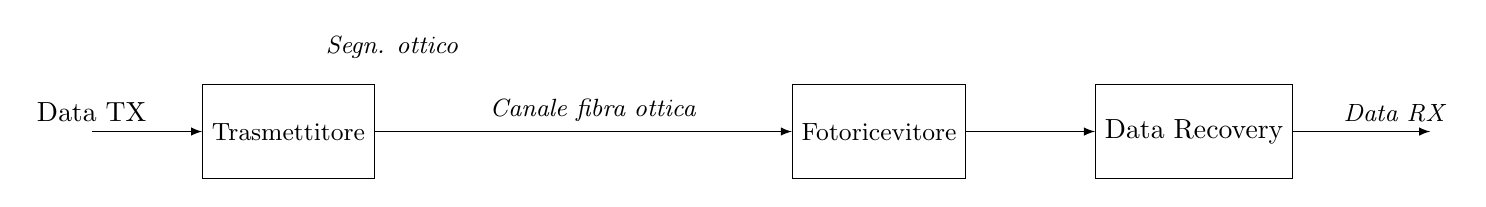
\begin{tikzpicture}[auto, node distance=2cm,>=latex']
	\node [input, name =input] {s(t)};
	\node[block, name = TRA, right of= input, node distance = 2.5cm]{\small{Trasmettitore}};
	\node[output, name = SEGN, right of =TRA, node distance = 2cm] {};
	\node[input, name = CAN, right of= SEGN, node distance = 2.5cm] {};
	\node[block, name = FOTO, right of = CAN, node distance =3cm] {\small{Fotoricevitore}};
`	\node[block, name = DATA, right of= FOTO, node distance = 4cm] {Data Recovery};
	\node[output, name = output, right of = DATA, node distance =3cm] {};
	
	\draw[-latex] (input.east) -- (TRA.west) node[at start, above]{Data TX};
	\draw[thin] (TRA.east) -- (SEGN.west) node[near start, above = 0.8cm]{\small{\textit{Segn. ottico}}};
	\draw[thin] (SEGN.east) -- (CAN.west) node[near end,above]{\small{\textit{Canale fibra ottica}}};
	\draw[-latex] (CAN.east) -- (FOTO.west);
	\draw[-latex] (FOTO.east) -- (DATA.west);
	\draw[-latex] (DATA.east) -- (output.west) node[near end, above]{\small{\textit{Data RX}}};

\end{tikzpicture}

\vspace{5mm}
L'onda luminosa portante può essere modulata secondo le modulazioni di: ampiezza (ASK Amplitude Shift Keying), fase (PSK Phase Shift Keying) e frequenza (FSK frequency Shift Keying).\\
Nella simulazione è implementata la ASK ON-OFF Non-Return-to-Zero.\\
Il segnale ottico trasmesso è definito dall'equazione:
\begin{equation}
	u(t) = \sqrt{2}a(t)\cos{[2\pi f_ct + \phi(t)]}
\end{equation}
con $f_c$ frequenza della portante.

Il segnale considerato è un segnale a banda stretta con banda \textit{B} tale che $B \ll f_c$.

Ciò ci consente di definire la rappresentazione complessa equivalente del segnale in banda base:
\begin{equation}
	\tilde{u}(t) = a(t)e^{i\phi(t)}
\end{equation}\
e dell'onda portante, defnita come:
\begin{equation}
	\tilde{c}(t) = \cos{(2\pi f_ct )}+ i\sin{(2\pi f_ct)} = e^{i2\pi f_c t}
\end{equation}

Per la ricezione del segnale si considera la potenza ottica ricevuta a valle del canale di trasmissione.
Questa è definita dal modulo quadro dell'inviluppo complesso:
\begin{equation}
	p(t) = |\tilde{u}(t)|^2 = a^2(t)
\end{equation}


\subsection{Canale di trasmissione}
\label{sub:Canale}

La risposta del canale è definita dalle caratteristiche del mezzo trasmissivo, in questo caso fibra di silice \textit{step-index}.
Per basse potenze ottiche (pochi mW) il suo comportamento è assimilabile a quello di un filtro lineare avente una funzione di trasferimento del tipo:
\begin{equation}
	H(f) = A(f) e^{j\beta(f)}
\end{equation}
dove:\begin{itemize}
	\item $A(f)$ è la risposta in ampiezza.
	\item $\beta(f)$ è la risposta in fase.
\end{itemize}

il segnale ottico all'uscita del canale è:
\begin{equation}
	u_{out}(t) = h(t) \ast u_{in}(t)
\end{equation}
Dato dalla convoluzione tra il segnale d'ingresso e la risposta impulsiva del canale.

Passando nel dominio della frequenza è possibile scrivere:
\begin{align*}
	U_{out}(f) &= H(f)U_{in}(f)\\
	H(f) &= \frac{U_{out}(f)}{U_{in}(f)}\\
\end{align*}

Il canale di trasmissione ha quindi un effetto di attenuazione dato dal termine $A(f)$ e di dispersione cromatica definita da $\beta(f)$.\\
Questi due termini rappresentano rispettivamente:
\begin{itemize}
	\item Coefficente di trasmissione in ampiezza
	\item Sfasamento del canale
\end{itemize}

% subsection  (end)


\subsection{Attenuazione}
\label{sub:attenuazione}

La perdita di potenza ottica costituisce uno dei fattori limitanti per il dimensionamento di linee di trasmissione in fibra ottica, in quanto riduce la potenza media del segnale ottico alla ricezione.

Le perdite sono condizionate da tre principali fattori:
\begin{enumerate}
	\item Perdita intrinseca e scattering di Rayleigh dati dalle caratteristiche fisiche del mezzo.
	\item Perdite dovute al \textit{microbending}.
	\item Perdite dovute allo \textit{splicing} (connessione cavi in serie).
\end{enumerate}

1. La perdita intrinseca consiste principalmente nell'assorbimento dovuto alle impurità di OH presenti nel mezzo (dovuti all'umidità inglobata nella matrice vetrosa). É una funzione di $\lambda^{-6}$, più è grande la lunghezza d'onda minore è la perdita.\\
Lo scattering  (cambiamento della direzione della radiazione) è dato dalla struttura molecolare disordinata del vetro ed è direttamente proporzionale a $\lambda^{-4}$.

Per il silicio si hanno tre finestre "ottime" per la trasmissione, la prima a 800 nm presenta attenuazione $\alpha = 1.5$ dB/Km, quelle usate più frequentemente sono le due a 1300 e 1550 nm, con tolleranze di 80 e 40 nm rispettivamente.
in queste ultime fasce si hanno coefficenti di attenuazione più bassi $\alpha = 0.35$ dB/km e $\alpha = 0.2 $ dB/km.


\begin{figure}[h!]
\centering
\includegraphics[scale=0.7]{attenuazione.png}
\caption{attenuazione nel silicio in funzione della lunghezza d'onda}
\end{figure}

2. Le piegature della fibra cambiano l'angolo di incidenza tra il fronte d'onda e il confine nucleo-matello. Oltre un certo raggio di curvatura può venire a mancare l'angolo d'incidenza minimo per avere riflessione totale.
Nel \textit{microbending} le perdite sono causate da imperfezioni sul fronte nucleo-mantello formatesi durante la produzione della fibra.

\vspace{5mm}
3. Durante lo splicing due parti di fibra sono unite tra loro fondendo le estremità. Se queste non sono state tagliate e allineate correttamente prima della fusione si possono verificare disturbi alla trasmissione del segnale.\\
Offset dell'alineamento del valore di $1\mu m$ possono produrre perdite significative. Il disturbo è quindi una fuzione della distanza tra gli assi dei cavi connessi.

\begin{figure}[h!]
\centering
\includegraphics[scale=0.4]{splicing.png}
\caption{disallineamento in due fibre ottiche}
\end{figure}

Ogni componente spettrale alla generica frequenza $f$ verrà attenuata con trasmittività in potenza:
\begin{equation}
	A^2(f) = |H(f)|^2 = \frac{|U_{out}(f)|^2}{|U_{in}(f)|^2}
\end{equation}

Il quadrato della risposta in ampiezza è una funzione esponenziale decrescente secondo la lunghezza L:
\begin{equation}
	A^2(f) = e^{-\alpha(f)L}  \rightarrow A(f) = e^{-\frac{1}{2}\alpha(f)L}
\end{equation}

$\alpha(f)$ è il \textbf{coefficiente d'attenuazione in potenza} in $[\frac{1}{Km}]$  (è preferibile la notazione in decibel), $A(f)$ risposta in ampiezza del canale.


Si definisce l'\textbf{Attenuazione} come l'inverso del coefficiente di trasmissione:
\begin{equation}\label{Q_eq}
	Q(f) = \frac{1}{A^2(f)} = e^{\alpha(f)L}
\end{equation}
Per la trasmissione considerata nel progetto con $\lambda = 1550 nm$ si considera $\alpha = 0.2 $ dB/Km.

\begin{equation}
	\alpha = \frac{0.2}{4.343} Km^{-1} = 0.046 Km^{-1} = 4.6*10^{-5} m^{-1}
\end{equation}

% subsection  (end)

\vspace{10mm}
\subsection{Dispersione cromatica}
\label{sub:dispersione}

La dispersione cromatica è dovuta al fatto che in fibra, frequenze diverse si propagano a velocità diverse. La principale causa è la dipendenza dell’indice di rifrazione dalla frequenza dell'onda.

L'effetto della dispersione è tanto più grande quanto è più largo lo spettro del segnale trasmesso.

\vspace{5mm}
La risposta in fase nell'intorno di $f_c$ può essere approssimata con lo sviluppo in serie di Taylor del secondo ordine:

\begin{equation}
	\beta(f) \cong \beta(f_c) + \frac{d\beta(f_c)}{df}(f-f_c) + \frac{1}{2}\frac{d^2\beta(f_c)}{df^2}(f-f_c)^2
\end{equation}

Esplicitando la dipendenza di $\beta(f)$ dalla lunghezza L del tratto di fibra ottengo tre parametri $\beta_0 , \beta_1, \beta_2$.

\begin{equation}
	\beta(f) \cong \beta_0(f_c)L + \beta_1(f_c)L*(f-f_c) + \frac{1}{2}\beta_2(f_c)L*(f-f_c)^2
\end{equation}

\begin{enumerate}
	\item Il termine di ordine 0 esprime la risposta in fase della portante:
	\begin{equation}
		\beta(f_c) = \beta_0(f_c)L
	\end{equation}
	
	Nella simulazione si considera $\beta_0$ costante uguale per tutte le frequenze. Poichè del segnale equivalente in banda base si considera solamente l'inviluppo, tale offset non influisce sul calcolo della risposta in fase del filtro di canale.
	
	Il ritardo di fase $\tau_p$ è il ritardo temporale (sec) della portante, uguale al numero di cicli della portante per la durata temporale di un suo ciclo.
	
	
	\begin{equation}
		\tau_p = \frac{\beta(f_c)}{2\pi f_c} = \frac{\beta_0(f_c)
		*L}{2\pi f_c}
	\end{equation}

	\item Il termine di ordine 1 contiene la derivata della risposta in frequenza valutata alla portante ed è legato al ritardo di gruppo $\tau_G$
	
	\begin{equation}
		\tau_G = \frac{\beta_1(f_c)*L}{2\pi}
	\end{equation}

		Il ritardo di gruppo indica il ritardo con cui l'energia dei segnali arriva al ricevitore, anch'esso non influisce sul calcolo delle prestazioni in quanto si considera che al ricevitore sia stato introdotto un meccanismo di recupero del sincronismo. 

	\item Il termine di ordine 2 è la derivata seconda della risposta in fase dle canale, è un indice della distorsione (espansione o compressione) dell'intervallo di trasmissione del bit.
	
	L'effetto di questo termine può essere compensato introducendo un tratto di canale detto \textit{Modulo di compensazione} realizzato con fibra speciale avente coeficiente di dispersione cromatica $D = -100\frac{\rho\text{s}}{\text{nm*Km}}$.
	
	Questa compensa la dispersione cromatica del canale, ma rappresenta un'ulteriore fonte di attenuazione del segnale.
	
	Considerando l'utilizzo di 1Km di fibra speciale ogni 6Km di fibra standard è possibile considerare nulla la risposta in fase del canale ($\beta(f) = 0$), a patto di introdurre un ulteriore termine d'attenuazione in potenza con coefficiente:
	\begin{equation}
		\alpha_{comp} = 0,5 \hspace{0.2cm} \text{dB/Km}
	\end{equation} 
		
\end{enumerate}

% subsection dispersione (end)

\subsection{Ricevitore a rivelazione diretta}
\label{sub:rice}


Il segnale giunto in fase di ricezione sarà caratterizzato dalla componente $a(t)$ (segnale dopo il filtro formatore)  la quale viene atenuata secondo $Q(f)$ (eq. \ref{Q_eq}) e subisce un ritardo di fase per l'effetto del filtro di canale $h_c(t)$.

\begin{equation}
	\tilde{u}_R(t) = a_R(t)e^{i\phi_r(t)}
\end{equation}

L'implementazione dei ricevitori ottici dipende dal formato di modulazione del segnale: analogico o digitale, On-Off keying o a livelli multipli.

Nel progetto si è implementato un sistema DD-OOK (Direct Detection ON/OFF keying).\\
Un sistema di ricezione ottica diretta, \textit{Fotoricevitore}, è costituito da:
\begin{itemize}
	\item Un \textbf{Fotodiodo}, il cui scopo è quello di convertire la potenza dell'onda luminosa [Watt] in corrente elettrica [Ampère], secondo un fattore detto \textit{responsivity} [A/W].
	La sua implementazione introduce rumore \textit{Shot}, prodotto dalle fluttuazioni casuali di natura quantistica della fotocorrente generata dal fotodiodo.\\
	Trattandosi di un rumore gaussiano bianco questo ha media nulla e deviazione standard:\\
	\begin{align*}
	\sigma_k^{shot} = \sqrt{2e\mu_kB_n}  \hspace{5mm}[A]
\end{align*}

	Dove $e = 1.6*10^{-19} $[C] è la carica elementare, $\mu_k$ è il valore medio del segnale elettrico corrispondente al bit k, $B_n =7.5 *10^9$[Hz] è la Banda equivalente di rumore.
	
	\item Un \textbf{TIA} Amplificatore a Transimpedenza, che converte la corrente a bassa intensità in una tensione [V], introducendo una componente di rumore \textit{Elettrico} determinata dal passaggio di corrente attraverso l'impedenza dell'amplificatore.
	Considerando il rumore equivalente in ingresso al TIA, questo risulta gaussiano bianco con media nulla e deviazione standard:
	\begin{align*}
	\sigma_n^{termico} = NEC\sqrt{B_n} \hspace{5mm} [A]
\end{align*}

	Dove il Rumore Equivalente di Corrente NEC$=20 \hspace{1.5mm}[\frac{\rho A}{\sqrt{Hz}}]$  e $B_n = 7.5 *10^9$[Hz].
	
\end{itemize}

\vspace{5mm}
Nella progettazione del sistema è stato considerato solamente l'effetto del rumore equivalente in ingresso al TIA.

%INSERIRE GRAFICO QUI!

\vspace{1cm}
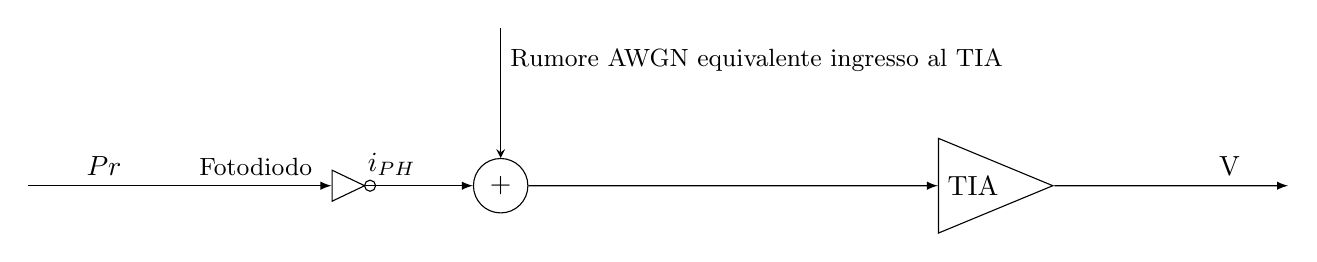
\begin{tikzpicture}[auto, node distance=2cm,>=latex']
	\node [input, name =input] {s(t)};
	\node[not gate US, draw, right of =input, node distance = 4cm](N1){};
	\node [sum, right of=N1] (sum) {+};
	\node[isosceles triangle, draw, right of= sum, node distance = 6cm](TIA) {TIA};
	\node [output, name=output, right of=TIA, node distance = 4cm] {};
	\node [input, name= input2, above of=sum, node distance=2cm] {};
	
	
	\draw[-latex] (input.east) -- (N1.west) node[near start,above]{$Pr$} node[near end,above]{\small{Fotodiodo}};
	\draw[-latex] (N1.east) -- (sum.west) node[near start ,above]{$i_{PH}$};
	\draw[-latex] (sum.east) -- (TIA.west) node[at end,above]{};
	\draw[-stealth] (input2.north) -- (sum.north) node[near start,right]{\small{Rumore AWGN equivalente ingresso al TIA}};
	\draw[-latex] (TIA.east) -- (output.west) node[near end, above]{V};
	
\end{tikzpicture}

% subsection  (end)

\subsection{Campionamento e decisore a soglia}
\label{sub:decisore}


Il segnale prima di essere campionato è nella forma:
\begin{align}
	r(t) = v(t) + n(t)
\end{align}
Dove $v(t)$ rappresenta la componente di segnale utile e $n(t)$ è la componente di rumore introdotta dall'Amplificatore.

I valori da inviare al decisore sono ottenuti campionando il segnale ricevuto a istanti (Ts/2 + kTs) con k intero [0; N -1], N numero di simboli. In questo modo il valore è letto nel punto di massimo al centro di ciascun intervallo di simbolo.

\begin{align}
	r_k = r(kTs + \frac{Ts}{2}) = v(kTs + \frac{Ts}{2}) + n(kTs + \frac{Ts}{2})
\end{align}

I valori ottenuti dal campionamento sono confrontati con il valore della soglia $\lambda$, definita come il valor medio del segnale, calcolato al ricevitore.

L'errore di trasmissione viene quantificato con il parametro BER \textit{bit error rate}, ovvero: 
\begin{align*}
	\text{BER} =  \frac{\text{n° bit errati}}{\text{n° bit trasmessi}}
\end{align*}

%CHIEDERE PARERE


\vspace{1cm}
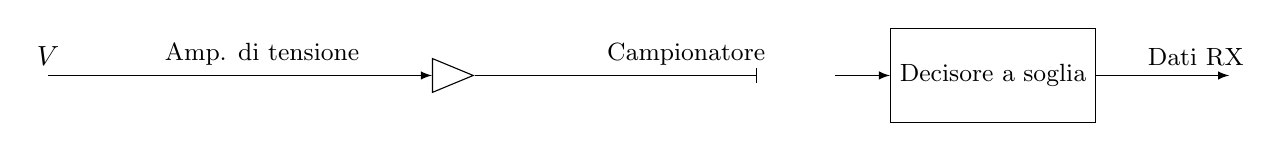
\begin{tikzpicture}[auto, node distance=2cm,>=latex']
	\node [input, name =input] {};
	\node[input, name =NameTia, right of= input, node distance =2cm]{Amp. di tensione}; 
	\node[isosceles triangle, draw, right of= NameTia, node distance = 3cm](TIA) {};
	\node[output, name=output1, right of=TIA, node distance = 4cm] {};
	\node[input, name = input2, right of= output1, node distance =1cm] {};
	\node[block, name= dec, right of= input2, node distance= 2cm] {\small{Decisore a soglia}};
	\node[output, name = output2, right of = dec, node distance = 3cm] {};
	
	
	\draw[thin] (input.east) -- (NameTia.west) node[at start,above]{$V$}; 
	\draw[-latex] (NameTia.east) -- (TIA.west) node[near start, above]{\small{Amp. di tensione}};
	\draw[-|] (TIA.east) -- (output1.west) node[near end, above]{\small{Campionatore}};
	\draw[-latex] (input2.east) -- (dec.west);
	\draw[-latex] (dec.east) -- (output2.west) node[near end, above]{\small{Dati RX}};
\end{tikzpicture}



% subsection  (end)

%Section end

\newpage
\section{Implementazione e codice Matlab}
\label{sec:2}

Il progetto è stato svolto attraverso il software \textbf{Matlab}.

\subsection{Definizione parametri principali}
\label{sub:2.1}

\begin{figure}[h!]
\centering
\includegraphics[scale=1.0]{parametri.png}
\caption{}
\label{}
\end{figure}

Variabili principali:
\begin{itemize}
	\item Lcanale\_Km: la lunghezza del canale in Km. 
	%CHIEDERE PER PROB. ERRORE
	\item LEN: numero di bit trasmessi
\end{itemize}

Vettore Tempo t\_s: definto da un valore 0 a fino al valore \textit{tempo\_totale} ottenuto dalla moltiplicazione tra numero di bit \textit{LEN} e il tempo di simbolo \textit{tsimbolo} $= 100 \rho$s. Con passo \textit{dt} $= 1 \rho$s.

\vspace{5mm}
Vettore Frequenze f\_s: definto da un valore 0 a fino al valore \textit{frequenza\_totale} ottenuto dal rapporto 1/\textit{dt}.  Con passo \textit{df} $= 1/$\textit{tempo\_totale}.

% subsection  (end)

\newpage
\subsection{Generazione del segnale}
\label{sub:2.2}

\begin{tikzpicture}[auto, node distance=2cm,>=latex']
	\node [input, name =input] {};
	\node[input, name =NameTia, right of= input, node distance =2cm]{Amp. di tensione}; 
	\node[block, draw, right of= NameTia, node distance = 1cm](GEN) {Gen. Sequenza Imp.};
	\node[input, name = input2, right of= output1, node distance =1cm] {};
	\node[block, name= REC, right of= GEN, node distance= 5cm] {\small{rect$(\frac{t-\frac{Tb}{2}}{Tb})$}};
	\node[block, name = SMO, right of = REC, node distance =4cm] {Filtro Smoothing};
	\node[output, name = output2, right of = dec, node distance = 3cm] {};
	
	
	\draw[-latex] (input.east) -- (GEN.west) node[at start, above]{dati binari};
	\draw[-latex] (GEN.east) -- (REC.west) node[near end, above = 0.9cm]{\small{Filtro formatore}};
	\draw[-latex] (REC.east) -- (SMO.west);
	\draw[-latex] (SMO.east) -- (output2.west) node[at end, above]{\small{Segnale \textit{TX} }};
\end{tikzpicture}

\vspace{5mm}
\begin{figure}[h!]
\centering
\includegraphics[scale=0.5]{sequenzabin.png}
\caption{}
\label{}
\end{figure}


La funzione \textit{randi} è utilizzata per generare un vettore di valori binari casuali di lunghezza \textit{LEN}.

Il primo ciclo For utilizza il vettore \textit{bit} per generare il segnale rettangolare con valori d'ampiezza 1 e 0 rispettivamente per i bit 1 e 0.

Per mantenere un rapporto d'estinzione lineare $\epsilon \cong 10$, il livello d'ampiezza 'basso' del bit 0 è stato posto a 1/sqrt(10). (Figura \ref{dig_sig}).
In questo caso
  \begin{figure}[h!]
  \centering
  \includegraphics[scale = 0.6]{digsig.png}
  \caption{segnale digitale di 16 bit}
  \label{dig_sig}
  \end{figure}


\newpage
\begin{figure}[h!]
\centering
\includegraphics[scale=0.4]{cosenorialzato.png}
\caption{}
\label{6}
\end{figure}

Poichè il segnale rettangolare generato è un'idealizzazione, ovvero non fisicamente realizzabile, si è implementato un filtro a coseno rialzato centrato in Ts.

Questo ha lo scopo di rendere le transizioni del segnale sinusoidali e non istantanee. 
Il filtro è definito di \textit{Smoothing}.

\begin{figure}[h!]
\centering
\includegraphics[scale=0.4]{convoluzionediscreta.png}
\caption{}
\label{}
\end{figure}

Attraverso l'uso della Fast Fourier Transform \textit{fft} si ottiene la risposta in frequenza del filtro, che moltiplicata per la trasformata del segnale digitale \textit{DIG\_SIG} definisce il segnale trasmesso \textit{TX} nel dominio della frequenza.

\vspace{5mm}
\begin{center}
\begin{tabular}{c c}
\includegraphics[scale = 0.7]{cosrialzatoimg.png}
&
\includegraphics[scale = 0.7]{segnalesmussato.png}
\end{tabular}
\end{center}

Il segnale viene poi traslato di mezzo periodo per compensare la traslazione dovuta agli effetti di bordo della convoluzione circolare con il coseno.

% subsection  (end)

\newpage
\subsection{Definizione della risposta del canale}
\label{sub:canalamatlab}


Vengono definite le risposte d'ampiezza \textbf{A(f)} e di fase $\boldsymbol{\beta(f)}$, equivalenti in banda base. 

\begin{itemize}
	\item $A^2(f)$ è considerato come il coefficiente di trasmissine in \textit{intensità} (potenza), perciò il suo effetto di attenuazione è calcolato in fase di ricezione.
	\item $\beta(f)$ introduce lo sfasamento del canale. 
\end{itemize}

\begin{figure}[h!]
\centering
\includegraphics[scale=0.7]{definizionecanal.png}
\caption{}
\label{}
\end{figure}
%%--------------------IMMAGINE---------------------------------

\textbf{Compensazione:}

\begin{figure}[h!]
\centering
\includegraphics[scale=0.7]{compensazione.png}
\caption{}
\label{}
\end{figure}


\textit{alpha\_specialdbkm} rappresenta l'attenuazione aggiuntiva in dB/Km introdotta dall'uso di 1 Km di fibra speciale ogni 6 Km di fibra regolare.

$A\_fspecial^2$ rappresenta il nuovo coefficiente di trasmissione in potenza complessivo.

\begin{figure}[h!]
\centering
\includegraphics[scale=0.7]{passaggiocanaleintesity.png}
\caption{}
\label{}
\end{figure}

\newpage
Si definisce la risposta in frequenza del canale \textit{Hc\_f0} simmetrica rispetto alla frequenza $f = 0$. Attraverso la \textit{fftshift} la si riporta nelle frequenze positive d'interesse. Il prodotto tra il segnale in ingresso e la risposta del canale nel dominio delle frequenze restituisce la risposta del segnale post canale \textit{RX}.



% subsection  (end)

\subsection{Fase di ricezione}
\label{sub:faseric}

In fase di ricezione il segnale è considerato sotto forma di potenza istantanea ricevuta \textit{rx\_intensity} (modulo quadro del segnale post canale).

Le componenti di potenza ricevuta $Prx\_bit1$ e $Prx\_bit0$  rispettivamente del bit 1 e 0 sono definite in relazione alla presenza o assenza del modulo di compensazione.

La fotocorrente \textit{I} è ottenuta moltiplicando la potenza istantanea per un valore di conversione\\ \textit{responsivity} [Ampère/Watt].

\begin{figure}[h!]
\centering
\includegraphics[scale=0.7]{faseric.png}
\label{}
\end{figure}

Il rumore gaussiano introdotto dal TIA è rappresentato dalla variabile \textit{w\_noise}, avente deviazione standard \textit{sigmateorica}.  Tale rumore è da considerarsi già filtrato.

%subsection (end)

\newpage
\subsection{Filtro a transimpedenza}
\label{sub:TIA}

La risposta del filtro a transimpedenza è di tipo gaussiano \textit{gaussian}, quest'ultima viene traslata per poter isolare la banda monolatera destra.

\begin{figure}[h!]
\centering
\includegraphics[scale=0.7]{filtrogaussiano.png}
\label{}
\end{figure}

\vspace{5mm}
\begin{center}
\begin{tabular}{c c}
\includegraphics[scale = 0.45]{gaussian.png}
&
\includegraphics[scale = 0.45]{gaussianshifted.png}
\end{tabular}
\end{center}

\vspace{1cm}
Il segnale in ingresso al TIA viene filtrato dal filtro gaussiano, mediante il prodotto nel dominio delle frequenze, per poi essere riportato nel dominio temporale \textit{rx\_tia}, dove viene sommata la componente di rumore \textit{w\_noise}. (Figura \ref{TIA})



\begin{figure}[h!]
\centering
\includegraphics[scale=0.7]{segnaletia.png}
\caption{}
\label{TIA}
\end{figure}

% subsection  (end)

\newpage
\subsection{Campionamento e decisore}
\label{sub:campionamento}

\begin{figure}[h!]
\centering
\includegraphics[scale=0.7]{campionamento.png}
\caption{}
\label{}
\end{figure}

La soglia di decisione è ottenuta calcolando la media dei valori ricevuti attraverso la funzione \textit{mean}.

Il confronto avviene con \textit{vettorecampioni}, ottenuto mediante il processo di campionamento.

I valori da inviare al decisore sono ottenuti campionando il segnale ricevuto a istanti (Ts/2 + kTs) con k intero [0; N -1], N numero di simboli. In questo modo il valore è letto nel punto di massimo al centro di ciscun intervallo di simbolo.

Il vettore \textit{bit\_stima} è il vettore dei valori stimati dal decisore.

\begin{figure}[h!]
\centering
\includegraphics[scale=0.7]{decide.png}
\caption{}
\label{}
\end{figure}

% subsection  (end)

\newpage
\subsection{SNR teorico e probabilità di bit errato stimata}
\label{sub:SNR}

Si è in grado di calcolare l'SNR teorico \textit{SNR} conoscendo la potenza ricevuta sui bit 1 e 0, e la varianza del rumore termico introdotto dal TIA.

Inoltre si definisce la probabilità di bit errato stimata utilizzando la funzione \textit{qfunc} applicata alla variabile \textit{Q}.

\begin{figure}[h!]
\centering
\includegraphics[scale=0.7]{SNR.png}
\caption{}
\label{}
\end{figure}

% subsection  (end)

\subsection{BER e eye diagram}
\label{sub:BER}

\vspace{3mm}
Il BER viene calcolato confrontando la sequenza dei bit stimati \textit{bit\_stima} con la sequenza di bit trasmessi \textit{bit}.

La variabile \textit{numerobiterrati} tiene conto del numero di confronti errati, divisa per il numero di bit totali \textit{LEN} restituisce il valore di BER.

\vspace{2mm}
\begin{figure}[h!]
\centering
\includegraphics[scale=0.7]{BER.png}
\caption{}
\label{}
\end{figure}

L'Eye diagram è ottenuto attraverso la ripetizione della funzione \textit{scatter}, che permette di tracciare su un grafico, sovrapposti in un unica finestra di ampiezza Ts, i valori del segnale ricevuto \textit{rx\_tia} per intervalli di tempo Ts successivi.

L'apertura verticale dell'Eye diagram è un indicatore della qualità della trasmissione: ad una maggiore ampiezza dell'occhio corrisponde un BER minore.

% subsection  (end)

% section  (end)


\newpage
\section{Risultati}
\label{sec:Ris}

\subsection{Analisi dei diagrammi ad occhio}
\label{sub:eye}

L'analisi del diagramma ad occhio consente di valutare rapidamente la qualità della trasmissione, di seguito si riportano gli eye diagram per i valori delle lunghezze di canale 0,40,60,90 Km.
In particolare si noti che, nella tabella \ref{tab:eye}: nel caso A non è presente la fibra speciale e di conseguenza si osserva l'effetto di dispersione cromatica; nel caso B invece, la compensazione è attiva, perciò l'effetto di dispersione è nullo, tuttavia l'attenuazione del segnale risulta superiore.



\begin{figure}[h!]
\centering
\includegraphics[scale=0.6]{compensazioneBERlen.jpg}
\caption{}
\label{BERcomp}
\end{figure}

Nel grafico a figura \ref{BERcomp} viene riportato l'andamento del BER in funzione della luncghezza in due casi differenti: 
\begin{itemize}
	\item Canale ON (Blu), senza modulo di compensazione, presenza di dispersione cromatica.
	\item Canale OFF (Rosso), fibra di compensazione attiva, assenza di dispersione cromatica.
\end{itemize}

Dopo circa 87 Km si osserva che l'effetto dell'attenuazione  complessiva dovuta alla fibra regolare e al modulo di compensazione ha un effetto di disturbo maggiore rispetto a quello dovuto all'attenuazione regolare più dispersione cromatica. (Figura \ref{BERcomp})

\newpage
\begin{table}[h!]
\centering
\begin{tabular}{ll}
\hline
CASO A & \multicolumn{1}{l}{CASO B} \\ \hline
0 Km   &                             \\ \hline
   \includegraphics[scale = 0.7]{OFF0.png}   &       \includegraphics[scale = 0.7]{ON0.png}                      \\ \hline
40 Km  &                             \\ \hline
   \includegraphics[scale = 0.7]{OFF40.png}       &     \includegraphics[scale = 0.7]{ON40.png}                         \\ \hline
60 Km  &                             \\ \hline
  \includegraphics[scale = 0.7]{OFF60.png}        &       \includegraphics[scale = 0.73]{ON60.png}                       \\ \hline
90 Km  &                             \\ \hline
    \includegraphics[scale = 0.7]{OFF90.png}   &              \includegraphics[scale = 0.73]{ON90.png}               
\end{tabular}
\caption{\label{tab:eye}Confronto degli eye diagram}
\end{table}


% subsection  (end)
\newpage
\subsection{BER e probabilità di bit errato teorica}
\label{sub:ber}


\begin{figure}[h!]
\centering
\includegraphics[scale=0.6]{probbiterrato.jpg}
\caption{}
\label{Pbe}
\end{figure}

Il Grafico in figura \ref{Pbe} riporta l'andamento del BER misurato in due casi distinti della simulazione, confrontandolo con l'andamento della probabailità di bit errato teorica.
\begin{itemize}
	\item Il primo caso (curva Blu) considera un rapporto d'estinzione $\epsilon$ pari a 10, ottenendo dunque una potenza trasmessa sul bit 0 pari a $P_{tx}^0 = P_{tx}^1/\epsilon $. Dove $P_{tx}^1 = 1$mA.
	\item Il secondo caso (curva Rossa) considera invece $\epsilon$ tendente a infinto, in modo da avere $P_{tx}^0 = 0$mA.
\end{itemize}

La curva Verde riporta la probabilità di bit errato teorica. Quest'ultima non è definita a partire dal campionamento e dagli errori verificati, ma è ottenuta tramite la \textit{qfunc} cosiderando solamente le potenze ricevute e la deviazione standard del rumore AWGN.  ($\epsilon \rightarrow \infty$).  

% subsection  (end)

% section  (end)


\end{document}